\documentclass[12pt]{article}
\usepackage{amsmath}
\usepackage{graphicx}
\usepackage{hyperref}
\usepackage[utf8]{inputenc}
\usepackage{geometry}
\usepackage{mathtools}
\usepackage{empheq}
\usepackage{listings}
\usepackage{xcolor}
\usepackage{minted}
\usepackage{svg}


\definecolor{LightGray}{gray}{0.9}

\graphicspath{ {./assets/} }
\geometry{margin=0.6in}

\title{CHEN 461 HW 6}
\author{Mark Levchenko}
\date{January 2023}

\begin{document}


\begin{enumerate}

% Problem 1 %%%%%%%%%%%%%%%%%%%%%%%%%%%%%%%%%%%%%%%%%%%%%%%%%%%%%%%%%%%%%%%%%%%%%%%%%%%
\newpage
\item Problem 6.13

\begin{align*}
    V \frac{dC_R}{dt} &= F (C_{R0} - C_R) - V k_1 C_R + V k_2 C_P - V k_3 C_R \\
    V \frac{dC_P}{dt} &= -F C_P + V k_1 C_R - V k_2 C_P \\
    \frac{dC_R}{dt} &= - \left(\frac{F}{V} + k_1 + k_3\right) C_R + k_2 C_P + \frac{F}{V} C_{R0} \\
    \frac{dC_P}{dt} &= k_1 C_R - \left(\frac{F}{V} + k_2\right) C_P \\
    y &= C_P \\
    A &= \begin{bmatrix}
        - \left(\frac{F}{V} + k_1 + k_3\right) & k_2 \\
        k_1 & - \left(\frac{F}{V} + k_2\right) \\
    \end{bmatrix} \\
    B &= \begin{bmatrix}
        \frac{F}{V} \\
        0 \\
    \end{bmatrix} \\
    C &= \begin{bmatrix}
        0 & 1 \\
    \end{bmatrix} \\
    D &= 0 \\
    G(s) &= c \left(s I - A\right)^{-1} b + d \\
    s I - A &= \begin{bmatrix}
        s + \left(\frac{F}{V} + k_1 + k_3\right) & - k_2 \\
        - k_1 & s + \left(\frac{F}{V} + k_2\right) \\
    \end{bmatrix} \\
    \mathrm{Adj}(s I - A) &= \begin{bmatrix}
        s + \left(\frac{F}{V} + k_2\right) & k_2 \\
        k_1 & s + \left(\frac{F}{V} + k_1 + k_3\right) \\
    \end{bmatrix} \\
    \mathrm{det}(s I - A) &= \left(s + \left(\frac{F}{V} + k_1 + k_3\right)\right) \left(s + \left(\frac{F}{V} + k_2\right)\right) - k_1 k_2 \\
    \mathrm{det}(s I - A) &= \left(s + \frac{F}{V} + k_1 + k_3\right) \left(s + \frac{F}{V} + k_2\right) - k_1 k_2 \\
    \theta &= \mathrm{det}(s I - A) \\
    \left(s I - A\right)^{-1} &= \theta^{-1} \begin{bmatrix}
        s + \left(\frac{F}{V} + k_2\right) & k_2 \\
        k_1 & s + \left(\frac{F}{V} + k_1 + k_3\right) \\
    \end{bmatrix} \\
    G(s) &= c \theta^{-1} \begin{bmatrix}
        s + \left(\frac{F}{V} + k_2\right) & k_2 \\
        k_1 & s + \left(\frac{F}{V} + k_1 + k_3\right) \\
    \end{bmatrix} \begin{bmatrix}
        \frac{F}{V} \\
        0 \\
    \end{bmatrix} \\
    G(s) &= c \theta^{-1} \begin{bmatrix}
        \frac{F}{V} \left(s + \left(\frac{F}{V} + k_2\right)\right) \\
        \frac{F}{V} k_1 \\
    \end{bmatrix} \\
    G(s) &= \theta^{-1} \begin{bmatrix}
        0 & 1 \\
    \end{bmatrix} \begin{bmatrix}
        \frac{F}{V} \left(s + \left(\frac{F}{V} + k_2\right)\right) \\
        \frac{F}{V} k_1 \\
    \end{bmatrix} \\
    G(s) &= \frac{\frac{F}{V} k_1}{\theta} \\
    \Aboxed{G(s) &= \frac{\frac{F}{V} k_1}{\left(s + \frac{F}{V} + k_1 + k_3\right) \left(s + \frac{F}{V} + k_2\right) - k_1 k_2}}
\end{align*}


% Problem 2 %%%%%%%%%%%%%%%%%%%%%%%%%%%%%%%%%%%%%%%%%%%%%%%%%%%%%%%%%%%%%%%%%%%%%%%%%%%
\newpage
\item Problem 6.7
\begin{enumerate}
    \item
    \begin{align*}
        \intertext{State space model:}
        A_1 \frac{dh_1}{dt} &= F_{in} - \frac{h_1 - h_2}{R_1} \\
        A_2 \frac{dh_2}{dt} &= \frac{h_1 - h_2}{R_1} - \frac{h_2}{R_2} \\
        \intertext{At steady state}
        0 &= 1 - \frac{1.5 - 0.5}{R_1} \\
        0 &= \frac{1.5 - 0.5}{R_1} - \frac{0.5}{R_2} \\
        R_1 &= 1 \\
        R_2 &= 0.5 \\
        \frac{dh}{dt} &= \begin{bmatrix}
            -\frac{1}{A_1 R_1} & \frac{1}{A_1 R_1} \\
            \frac{1}{A_2 R_1} & -\left(\frac{1}{A_2 R_1}+\frac{1}{A_2 R_2}\right)
        \end{bmatrix} h + \begin{bmatrix}
            \frac{1}{A_1} \\
            0 \\
        \end{bmatrix} F_{in} \\
        y &= \begin{bmatrix}
            0 & 1 \\
        \end{bmatrix} h \\
        A &= \begin{bmatrix}
            -1 & 1 \\
            0.5 & -1.5 \\
        \end{bmatrix} \\
        B &= \begin{bmatrix}
            1 \\
            0 \\
        \end{bmatrix} \\
        h(0) &= \begin{bmatrix}
            1.5 \\
            0.5 \\
        \end{bmatrix} \\
        \intertext{Simulate response with lsim}
        D &= 0 \\
        \intertext{For $h_1$ response}
        C &= \begin{bmatrix}
            1 & 0 \\
        \end{bmatrix} \\
        \intertext{For $h_2$ response}
        C &= \begin{bmatrix}
            0 & 1 \\
        \end{bmatrix}
    \end{align*}    

    Simulate a response to an unforced input on the system. The initil heights are supplied as the initial condition.

    Simulated response plot:

    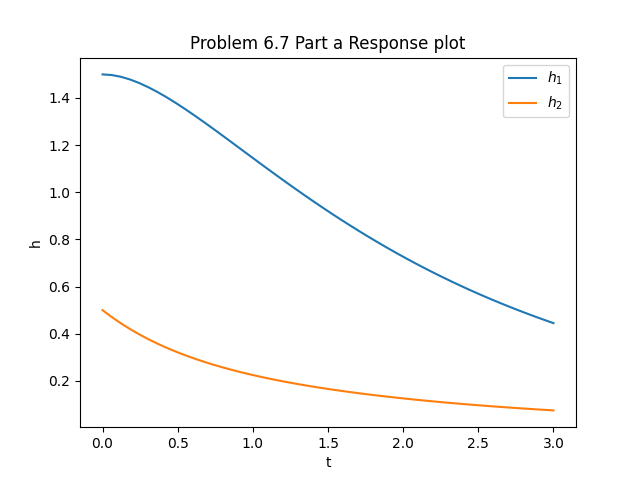
\includegraphics{assets/p2_a.png}

    The plot was generated with the code below:

\begin{minted}[
framesep=2mm,
baselinestretch=1.2,
bgcolor=LightGray,
fontsize=\footnotesize,
breaklines,
]{python}
import numpy as np
import matplotlib.pylab as plt
from scipy.signal import lti, step, lsim

h_1_0 = 1.5
h_2_0 = 0.5

A = np.array([
    [-1, 1],
    [.5, -1.5]
])
B = np.array([
    [1],
    [0]
])
C_h1 = np.array([1, 0])
C_h2 = np.array([0, 1])
D = 0

sys_h1 = lti(A, B, C_h1, D)
sys_h2 = lti(A, B, C_h2, D)

# Part A
u = 0
t = np.linspace(0, 3, 50)

t_h1_a, h1_a, x1 = lsim(sys_h1, u, t, h_1_0)
t_h2_a, h2_a, x2 = lsim(sys_h2, u, t, h_2_0)

plt.plot(t_h1_a, h1_a, label=r"$h_1$")
plt.plot(t_h2_a, h2_a, label=r"$h_2$")
plt.xlabel(r"t")
plt.ylabel(r"h")
plt.title("Problem 6.7 Part a Response plot")
plt.legend()
plt.show()

# Part B
t_react = np.interp(0.2, np.flip(h2_a), np.flip(t_h2_a))
h_1_react = np.interp(t_react, t_h1_a, h1_a)
print(f"Time when h_2 = 0.2 m: {t_react} min")
print(f"h_1 at that time: {h_1_react}")

# Part C
t_h1_c, h1_c = step(sys_h1, X0=h_1_react)
t_h2_c, h2_c = step(sys_h2, X0=0.2)

plt.plot(t_h1_c, h1_c, label=r"$h_1$")
plt.plot(t_h2_c, h2_c, label=r"$h_2$")
plt.xlabel(r"t")
plt.ylabel(r"h")
plt.title("Problem 6.7 Part c Response plot")
plt.legend()
plt.show()

print(f"Final h_1 = {h1_c[-1]}")
print(f"Final h_2 = {h2_c[-1]}")
\end{minted}

\item To find the the time that $h_2 = 0.2$ m, the output arrays for the $h_2$ response were interpolated. With the time value, $h_1$ at that time was also interpolated from the $h_1$ response arrays. The code above shows the interpolation and output.

$h_2$ reaches 0.2 m at $\boxed{1.1845 \text{min}}$.

At that time, $h_1$ is $\boxed{1.0594 \text{m}}$.

\item To find the response of the heights when the flow is restored, another response simulation was made. The flow switching on is equivalent to a step response, and so a step response to the system will be simulated. The code above also contains the code for this simulation. 

Response plot:

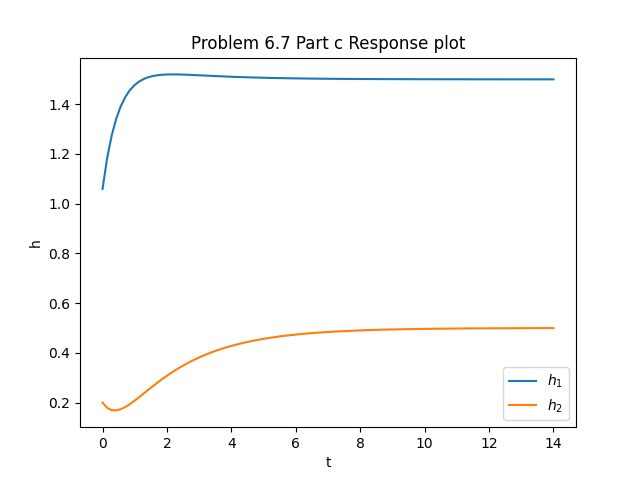
\includegraphics{assets/p2_c.png}

$h_1$ ends up at 1.5 m, and $h_2$ ends up at 0.5 m. Both heights return to their steady state values.
\end{enumerate}


% Problem 3 %%%%%%%%%%%%%%%%%%%%%%%%%%%%%%%%%%%%%%%%%%%%%%%%%%%%%%%%%%%%%%%%%%%%%%%%%%%
\newpage
\item Problem 6.8
\begin{enumerate}
    \item 
    \begin{align*}
        \tau \frac{dx_1}{dt} + x_1 &= ku \\
        \tau \frac{dx_2}{dt} + x_2 &= kx_1 \\
        \frac{dx_1}{dt} &= -\frac{x_1}{\tau} + \frac{k}{\tau} u \\
        \frac{dx_2}{dt} &= \frac{k}{\tau} x_1 - \frac{x_2}{\tau} \\
        A &= \begin{bmatrix}
            -\frac{1}{\tau} & 0 \\
            \frac{k}{\tau} & -\frac{1}{\tau} \\
        \end{bmatrix} \\
        B &= \begin{bmatrix}
            \frac{k}{\tau} \\
            0 \\
        \end{bmatrix} \\
        sI-A &= \begin{bmatrix}
            s+\frac{1}{\tau} & 0 \\
            -\frac{k}{\tau} & s+\frac{1}{\tau} \\
        \end{bmatrix} \\
        \mathrm{Adj}(sI-A) &= \begin{bmatrix}
            s+\frac{1}{\tau} & 0 \\
            \frac{k}{\tau} & s+\frac{1}{\tau} \\
        \end{bmatrix} \\
        \mathrm{det}(sI-A) &= (s+\frac{1}{\tau})^2 \\
        (sI-A)^{-1} &= \begin{bmatrix}
            \frac{1}{s+1/\tau} & 0 \\
            \frac{\tau k}{\tau^2s^2+2\tau s + 1} & \frac{1}{s+1/\tau} \\
        \end{bmatrix} \\
        \mathcal{L}^{-1}\left\{(sI-A)^{-1}\right\} &= \begin{bmatrix}
            e^{-t/\tau} & 0 \\
            \frac{k}{\tau} t e^{-t/\tau} & e^{-t/\tau} \\
        \end{bmatrix} \\
        e^{At} &= \begin{bmatrix}
            e^{-t/\tau} & 0 \\
            \frac{k}{\tau} t e^{-t/\tau} & e^{-t/\tau} \\
        \end{bmatrix} \\
    \end{align*}
    \item 
    \begin{align*}
        x(t) &= \begin{bmatrix}
            0 & 1 \\
        \end{bmatrix} \begin{bmatrix}
            e^{-t/\tau} & 0 \\
            \frac{k}{\tau} t e^{-t/\tau} & e^{-t/\tau} \\
        \end{bmatrix} \begin{bmatrix}
            x_1(0) \\
            x_2(0) \\
        \end{bmatrix} \\
        x(t) &= \begin{bmatrix}
            e^{-t/\tau} x_1(0) \\
            \frac{k}{\tau} t e^{-t/\tau} x_1(0) + e^{-t/\tau} x_2(0) \\
        \end{bmatrix}
    \end{align*}
    \item 
    \begin{align*}
        A_d &= \begin{bmatrix}
            e^{-T_s/\tau} & 0 \\
            \frac{k}{\tau} T_s e^{-T_s/\tau} & e^{-T_s/\tau} \\
        \end{bmatrix} \\
        B_d &= \int_0^{T_s} e^{At} B dt \\
        e^{At} B &= \begin{bmatrix}
            e^{-t/\tau} & 0 \\
            \frac{k}{\tau} t e^{-t/\tau} & e^{-t/\tau} \\
        \end{bmatrix} \begin{bmatrix}
            \frac{k}{\tau} \\
            0 \\
        \end{bmatrix} \\
        e^{At} B &= \begin{bmatrix}
            \frac{k}{\tau} e^{-t/\tau} \\
            \frac{k^2}{\tau^2} t e^{-t/\tau} \\
        \end{bmatrix} \\
        B_d &= \int_0^{T_s} \begin{bmatrix}
            \frac{k}{\tau} e^{-t/\tau} \\
            \frac{k^2}{\tau^2} t e^{-t/\tau} \\
        \end{bmatrix} dt \\
        B_d &= \begin{bmatrix}
            -k e^{-t/\tau} \\
            \frac{k^2}{\tau} \left(- \tau t e^{-t/\tau} - \tau^2 e^{-t/\tau}\right) \\
        \end{bmatrix} \\
    \end{align*}
\end{enumerate}


% Problem 4 %%%%%%%%%%%%%%%%%%%%%%%%%%%%%%%%%%%%%%%%%%%%%%%%%%%%%%%%%%%%%%%%%%%%%%%%%%%
\newpage
\item MATLAB Problem

\begin{enumerate}
    \item 
    \begin{align*}
        \frac{d}{dt} \begin{bmatrix}
            C_R \\
            C_I \\
            C_P \\
        \end{bmatrix} &= \begin{bmatrix}
            -\left(\frac{F}{V} + k_1\right) & 0 & 0 \\
            k_1 & -\left(\frac{F}{V} + k_2\right) & k_3 \\
            0 & k_2 & -\left(\frac{F}{V} + k_3\right) \\
        \end{bmatrix} \begin{bmatrix}
            C_R \\
            C_I \\
            C_P \\
        \end{bmatrix} + \begin{bmatrix}
            \frac{F}{V} \\
            0 \\
            0 \\
        \end{bmatrix} C_{R0} \\
        & k_1 = 0.1 \\
        & k_2 = 0.05 \\
        & k_3 = 0.02 \\
        & F = 10 \\
        & V = 100 \\
        & \frac{F}{V} = 0.1 \\
        & C_{R0,s} = 2 \\
        A &= \begin{bmatrix}
            -\left(0.1 + 0.1\right) & 0 & 0 \\
            0.1 & -\left(0.1 + 0.05\right) & 0.02 \\
            0 & 0.5 & -\left(0.1 + 0.02\right) \\
        \end{bmatrix} \\
        A &= \begin{bmatrix}
            -0.2 & 0 & 0 \\
            0.1 & -0.15 & 0.02 \\
            0 & 0.5 & -0.12 \\
        \end{bmatrix} \\
        Bu &= \begin{bmatrix}
            0.1 \\
            0 \\
            0 \\
        \end{bmatrix} \cdot 2 \\
        Bu &= \begin{bmatrix}
            0.2 \\
            0 \\
            0 \\
        \end{bmatrix} \\
        \intertext{At steady state:}
        0 &= Ax + Bu \\
        x &= -A^{-1} Bu \\
        x &= -\begin{bmatrix}
            -0.2 & 0 & 0 \\
            0.1 & -0.15 & 0.02 \\
            0 & 0.5 & -0.12 \\
        \end{bmatrix}^{-1} \begin{bmatrix}
            0.2 \\
            0 \\
            0 \\
        \end{bmatrix} \\
        x &= \begin{bmatrix}
            1 \\
            0.7059 \\
            0.2941 \\
        \end{bmatrix} \\
        C_R &= 1 \\
        C_I &= 0.7059 \\
        C_P &= 0.2941
    \end{align*}
    \item Response plots:
    
    Step response:

    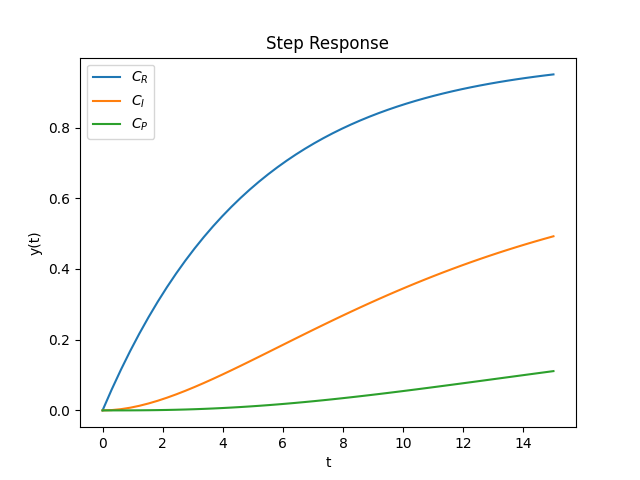
\includegraphics{assets/p4_step.png}

    Ramp response: 

    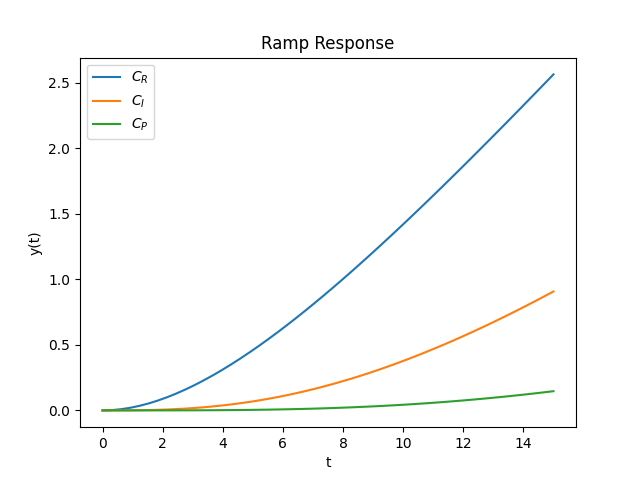
\includegraphics{assets/p4_ramp.png}

    Sinusoidal response:

    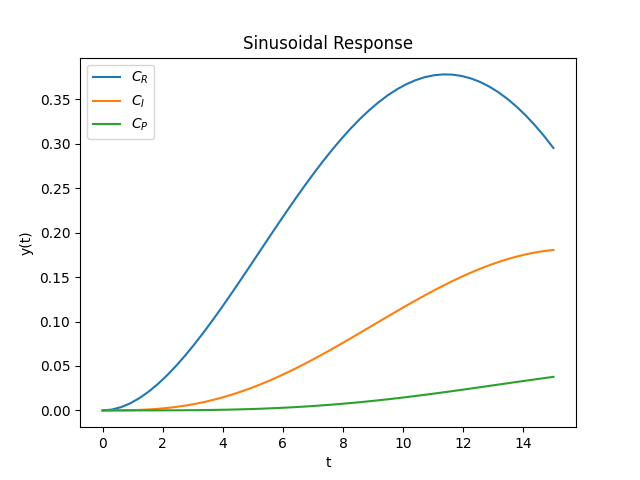
\includegraphics{assets/p4_sin.png}

    Code for creating the plots and calculating zero hold disretization:

\begin{minted}[
framesep=2mm,
baselinestretch=1.2,
bgcolor=LightGray,
fontsize=\footnotesize,
breaklines,
]{python}
import numpy as np
from scipy import linalg, signal
import matplotlib.pylab as plt
import math

import pprint


def steady_state_composition(A, B) -> None:
    C_R0s = 2

    Bu = B * C_R0s

    steady_state_solution = -linalg.solve(A, Bu)

    print(steady_state_composition)


def step_response(t, M, A, B, c):
    step_response_formula = lambda t: M * (c @ (linalg.expm(A * t) - np.eye(3)) @ linalg.inv(A) @ B)
    response = np.zeros(len(t))

    for i, val in enumerate(t):
        response[i] = step_response_formula(val)[0]

    return response


def ramp_response(t, M, A, B, c):
    ramp_response_formula = lambda t: M * (c @ ((linalg.expm(A * t) - np.eye(3)) @ linalg.inv(A) - t * np.eye(3)) @ linalg.inv(A) @ B)
    response = np.zeros(len(t))

    for i, val in enumerate(t):
        response[i] = ramp_response_formula(val)[0]

    return response


def sinusoidal_response(t, M, omega, A, B, c):
    sinusoidal_response_formula = lambda t: c @ (omega * linalg.expm(A * t) - A * math.sin(omega * t) - omega * np.eye(3) * math.cos(omega * t)) @ linalg.inv(np.linalg.matrix_power(A, 2) + omega**2 * np.eye(3)) @ B * M
    response = np.zeros(len(t))

    for i, val in enumerate(t):
        response[i] = sinusoidal_response_formula(val)[0]

    return response

def plot_step_response(A, B):
    M = 2

    c_C_R = np.array([1, 0, 0])
    c_C_I = np.array([0, 1, 0])
    c_C_P = np.array([0, 0, 1])

    t_plot = np.linspace(0, 15, 50)

    plt.plot(t_plot, step_response(t_plot, M, A, B, c_C_R))
    plt.plot(t_plot, step_response(t_plot, M, A, B, c_C_I))
    plt.plot(t_plot, step_response(t_plot, M, A, B, c_C_P))
    plt.title("Step Response")
    plt.xlabel("t")
    plt.ylabel("y(t)")
    plt.legend([r"$C_R$", r"$C_I$", r"$C_P$"])
    plt.show()


def plot_ramp_response(A, B):
    M = 0.5

    c_C_R = np.array([1, 0, 0])
    c_C_I = np.array([0, 1, 0])
    c_C_P = np.array([0, 0, 1])

    t_plot = np.linspace(0, 15, 50)

    plt.plot(t_plot, ramp_response(t_plot, M, A, B, c_C_R))
    plt.plot(t_plot, ramp_response(t_plot, M, A, B, c_C_I))
    plt.plot(t_plot, ramp_response(t_plot, M, A, B, c_C_P))
    plt.title("Ramp Response")
    plt.xlabel("t")
    plt.ylabel("y(t)")
    plt.legend([r"$C_R$", r"$C_I$", r"$C_P$"])
    plt.show()


def plot_sinusoidal_response(A, B):
    M = 1 
    omega = 0.2

    c_C_R = np.array([1, 0, 0])
    c_C_I = np.array([0, 1, 0])
    c_C_P = np.array([0, 0, 1])

    t_plot = np.linspace(0, 15, 50)

    plt.plot(t_plot, sinusoidal_response(t_plot, M, omega, A, B, c_C_R))
    plt.plot(t_plot, sinusoidal_response(t_plot, M, omega, A, B, c_C_I))
    plt.plot(t_plot, sinusoidal_response(t_plot, M, omega, A, B, c_C_P))
    plt.title("Sinusoidal Response")
    plt.xlabel("t")
    plt.ylabel("y(t)")
    plt.legend([r"$C_R$", r"$C_I$", r"$C_P$"])
    plt.show()


def main():
    k_1 = 0.1 
    k_2 = 0.05
    k_3 = 0.02
    F = 10 
    V = 100

    A = np.array([
        [-(F / V + k_1), 0, 0],
        [k_1, -(F / V + k_2), k_3],
        [0, k_2, -(F / V + k_3)],
    ])

    B = np.array([
        [F/V],
        [0],
        [0],
    ]) 

    steady_state_composition(A, B)


    plot_step_response(A, B)


    plot_ramp_response(A, B)


    plot_sinusoidal_response(A, B)

    C = np.array([1, 1, 1])
    D = 0
    sys = signal.lti(A, B, C, D)

    pp = pprint.PrettyPrinter(indent=4)

    pp.pprint(signal.cont2discrete((A, B, C, D), 0.2))

if __name__ == "__main__":
    main()
\end{minted}

    \item Zero hold discretization was calulated with the code in the previous part.
    
    \begin{align*}
        A_d &= \begin{bmatrix}
            0.960789439 & 0 & 0 \\
            0.0193123181 & 0.970464981 & 3.89347676\cdot10^{-5} \\
            9.69160980\cdot10^{-5} & 9.73369191\cdot10^{-3} & 0.976305197 \\
        \end{bmatrix} \\
        B_d &= \begin{bmatrix}
            0.0196052804 \\
            1.95395071\cdot10^{-4} \\
            6.51198080\cdot10^{-7} \\
        \end{bmatrix}
    \end{align*}
    % rray([[9.60789439e-01, 0.00000000e+00, 0.00000000e+00],
    %    [1.93123181e-02, 9.70464981e-01, 3.89347676e-03],
    %    [9.69160980e-05, 9.73369191e-03, 9.76305197e-01]]),
    % array([[1.96052804e-02],
    %    [1.95395071e-04],
    %    [6.51198080e-07]])
\end{enumerate}

\end{enumerate}
\end{document}